

\documentclass[a4paper]{article}

\usepackage{amsmath}
\usepackage{hyperref}
\usepackage{biblatex}
\usepackage{enumerate}
\usepackage{graphicx}
\usepackage{stmaryrd}
\usepackage[dvipsnames]{xcolor}
\usepackage{listings}
\usepackage{caption}
\usepackage{subcaption}
\usepackage{booktabs}
\usepackage{float}

\addbibresource{refs.bib}

\begin{document}

\author{Ola Bratt \\
  \href{mailto:ola.bratt@gmail.com}{ola.bratt@gmail.com}
  \and
  Patrick Attimont \\
  \href{patrickattimont@gmail.com}{patrickattimont@gmail.com}
}

\title{DAT565/DIT407 Assignment 5}
\date{2024-02-xx}

\maketitle

This paper is addressing the assignment 3 study queries within the \emph{Introduction to Data Science \& AI} course, DIT407 at 
the University of Gothenburg and DAT565 at Chalmers. The main source of information for this project
is derived from the lectures and Skiena~\cite{Skiena:2024}. Assignment 5 is about distance and network methods.

\section*{Problem 1: Preprocessing the dataset}

\section*{Problem 2: Determining the appropriate number of clusters}

\begin{figure}[H]
  \begin{center}
    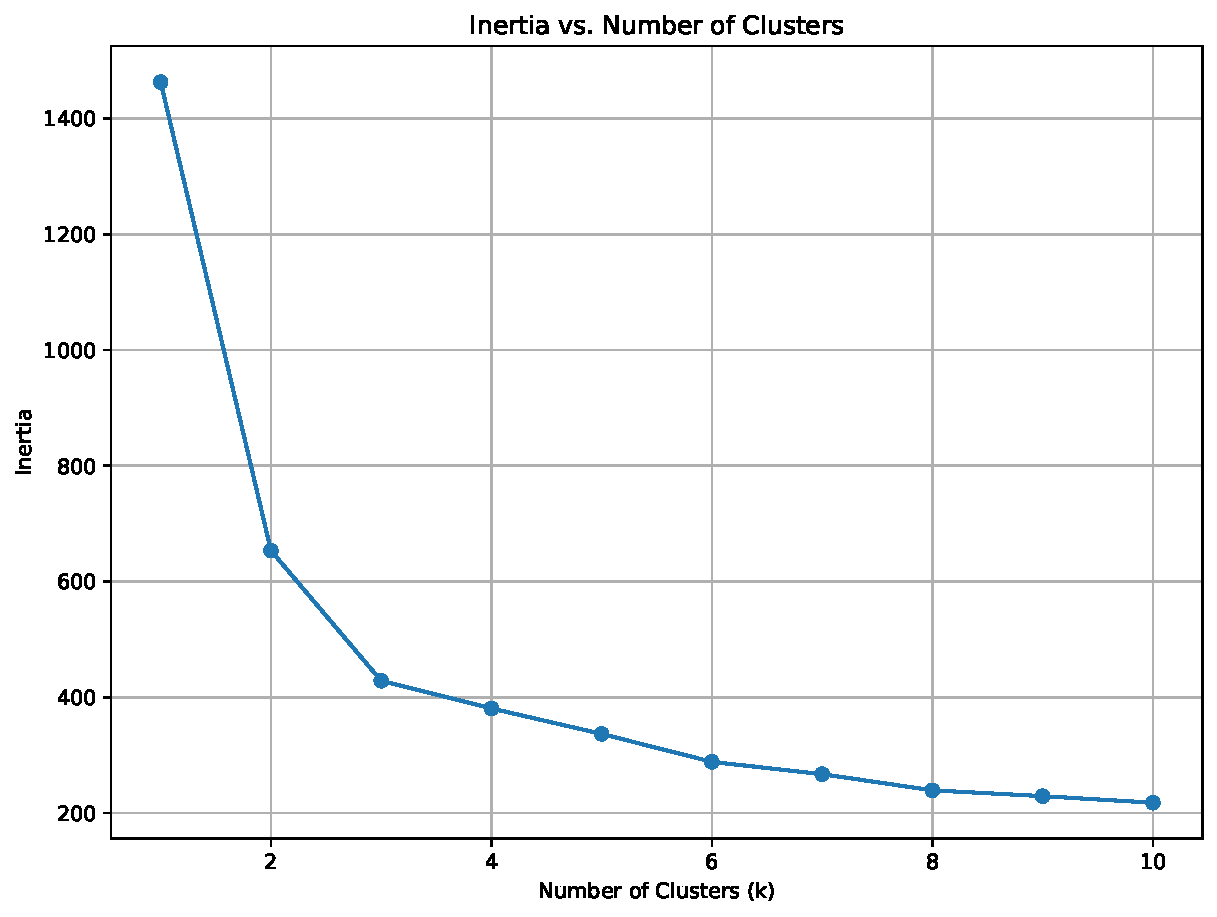
\includegraphics[width=\textwidth]{ola/intertia.pdf}
    \caption{Invertia vs. Number of clusters}
    \label{fig:inertia}
  \end{center}
\end{figure}

\section*{Problem 3: Visualizing the classes}

\begin{figure}[H]
  \begin{center}
    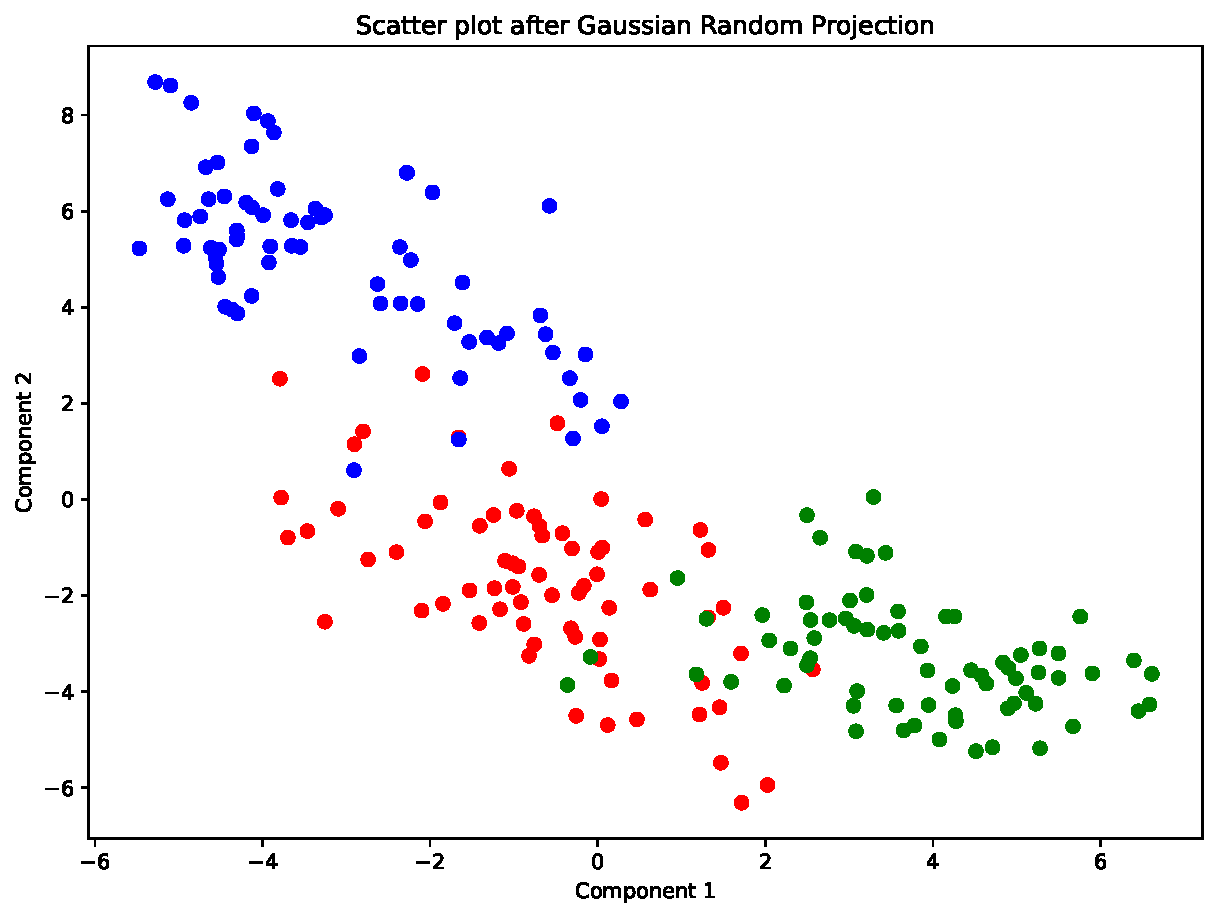
\includegraphics[width=\textwidth]{ola/gaussian_random_projection.pdf}
    \caption{Gaussian random projection}
    \label{fig:gaussian_random_projection}
  \end{center}
\end{figure}

\begin{figure}[H]
  \begin{center}
    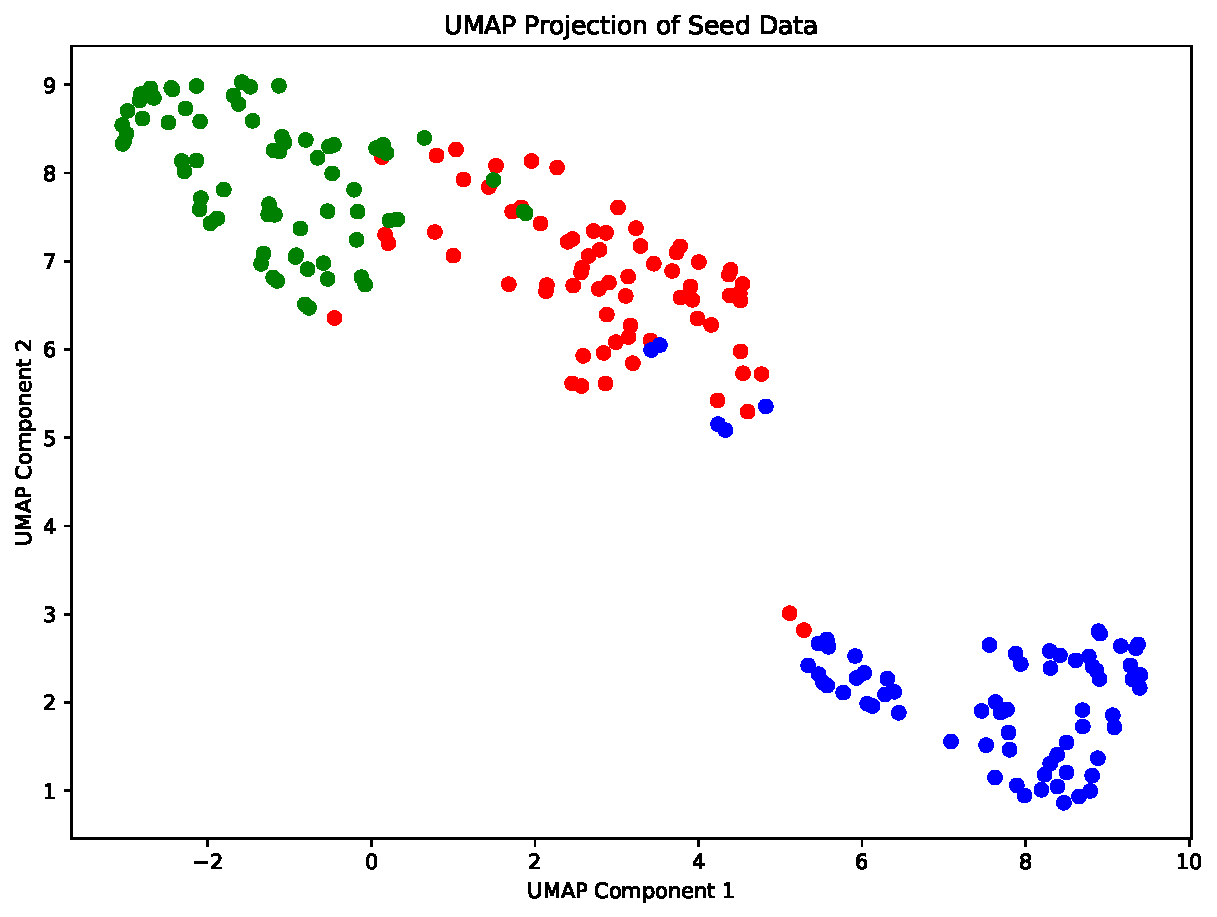
\includegraphics[width=\textwidth]{ola/umap.pdf}
    \caption{UMAP projection of Seeds}
    \label{fig:umap}
  \end{center}
\end{figure}

\section*{Problem 4: Evaluating clustering}
To apply \textit{k}-means clustering to the data, we use the \verb|KMeans| function from \verb|sklearn| with 3 as the number of clusters, and then build the model on the normalized data.

The rand index is obtained by applying the \verb|rand_score| function on the labels of the clustering and the true labels. Its value is 0.90.

Finally we iterate over all the possible permutations in the range $ [0\ldotp\ldotp4] $ to find the best accuracy score. With the permutation $\{0, 1, 2, 3\} \rightarrow \{2, 3, 1, 0\}$, the accuracy is equal to 0.92.

\section*{Problem 5: Agglomerative clustering}
We iterate over the linkage options and calculate the accuracy value after finding the right permutation. The best linkage option is the ward method.

\begin{figure}[H]
  \begin{center}
    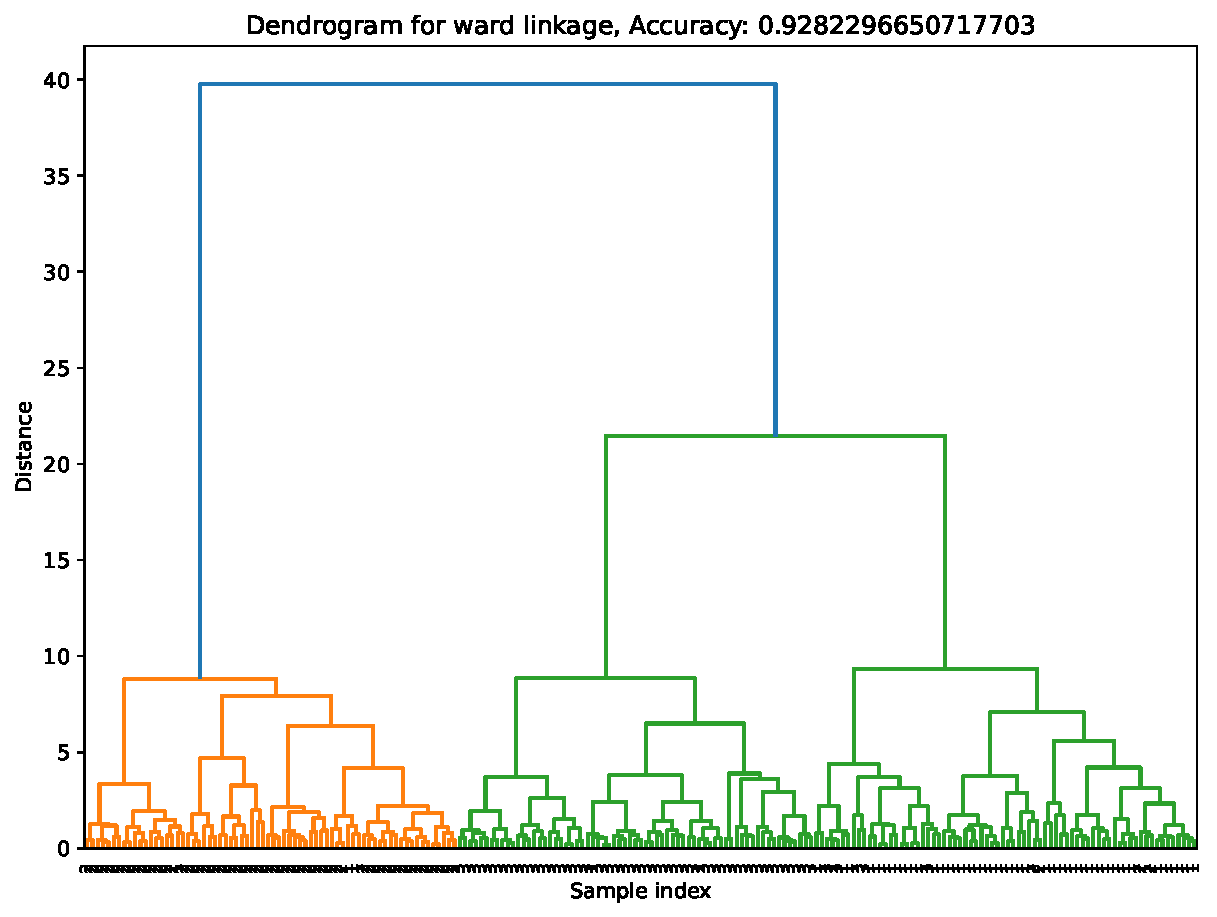
\includegraphics[width=\textwidth]{ola/dendrogram.pdf}
    \caption{Dendrogram}
    \label{fig:dendrogram}
  \end{center}
\end{figure}

\newpage


\printbibliography

\section*{Appendix: Source Code}

\lstset{
  language=Python,
  basicstyle=\ttfamily,
  commentstyle=\color{OliveGreen},
  keywordstyle=\bfseries\color{Magenta},
  stringstyle=\color{YellowOrange},
  numbers=left,
  basicstyle=\footnotesize,
  breaklines=true,
  postbreak=\mbox{\textcolor{red}{$\hookrightarrow$}\space}
}


\lstinputlisting{ola/assignment5.py}

\end{document}
